\section{Ejercicio 1}
\subsection{El Problema}

Se tiene un grafo $G$ $=$ $(V,E)$ de N vértices y M ejes bidireccionales. Se tienen además dos subconjuntos disjuntos $A \subset V$ y $Esc \subset V$ que representan alumnos y escuelas respectivamente. El problema consiste en encontrar la cantidad mínima de vértices $D$ (que representan divulgadores)  tales que para cualquier camino $C$ que una un vértice de $A$ con un vértice de $Esc$, algún $d_i \in C$. Se pide implementar un algoritmo que resuelva este problema con complejidad temporal $O(NM^2)$

\subsection{Desarrollo}

Se pensó el problema utilizando la idea de corte mínimo. Esto es, se quería buscar el corte mínimo tal que los ejes de $A$ queden de un lado y los de $Esc$ del otro. Para esto se armó una red de flujo, agregando dos vértices $s$ y $t$ (sumidero y fuente respectivamente). Se conectó $s$ a los vértices de $A$ y $t$ a los de $Esc$. Se decidió ponerle capacidad 1 a todos los ejes. De esta forma se pensó en, obteniendo el corte mínimo, ver la mínima cantidad de ejes que separan los vértices de $A$ de los de $Esc$. Esto sería equivalente a obtener el flujo máximo, por el teorema de $max-flow$ $min-cut$. Tras discutir esta idea se llegó a un ejemplo que mostró que esa solución no era la indicada.

%%Insertar acá grafo de ejemplo, cuando tenga la herramienta%%

\begin{figure}[H]
\centering
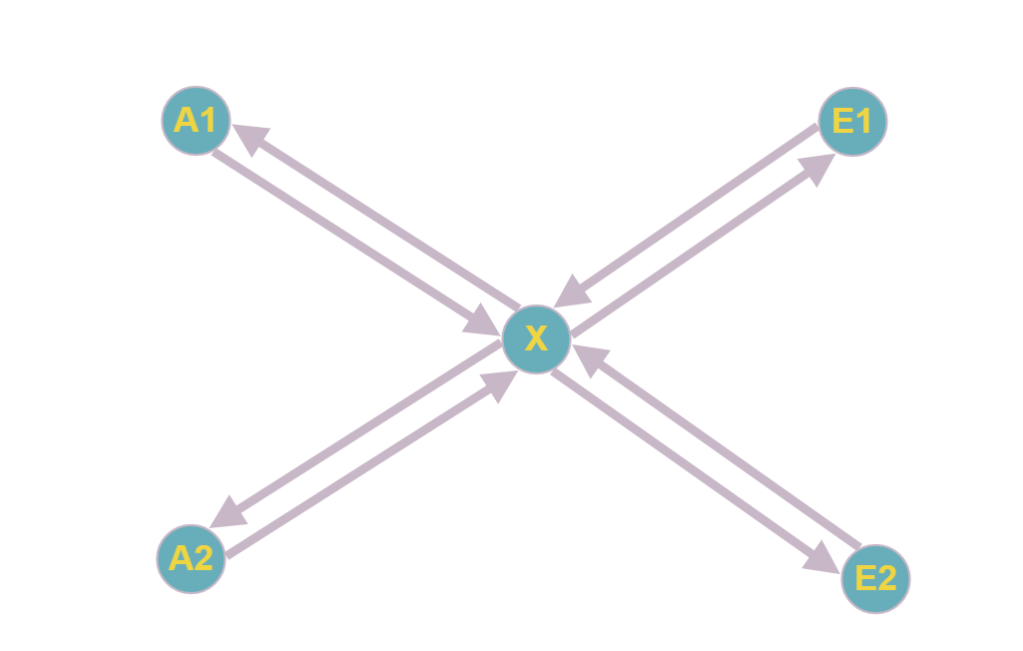
\includegraphics[width=15cm]{Imagenes/Ej1a.png}
\caption{Grafo 1}
\end{figure}

En el Grafo 1, se puede ver que hay dos alumnos, dos escuelas, y una esquina intermedia. La correcta solución al problema sería poner un divulgador en la esquina central, vértice $X$ en la imagen. Al armar la red de flujo quedaría el Grafo 2. Asumir que todas las capacidades de los ejes son 1. No están en la imagen para no ensuciarla.

\begin{figure}[H]
\centering
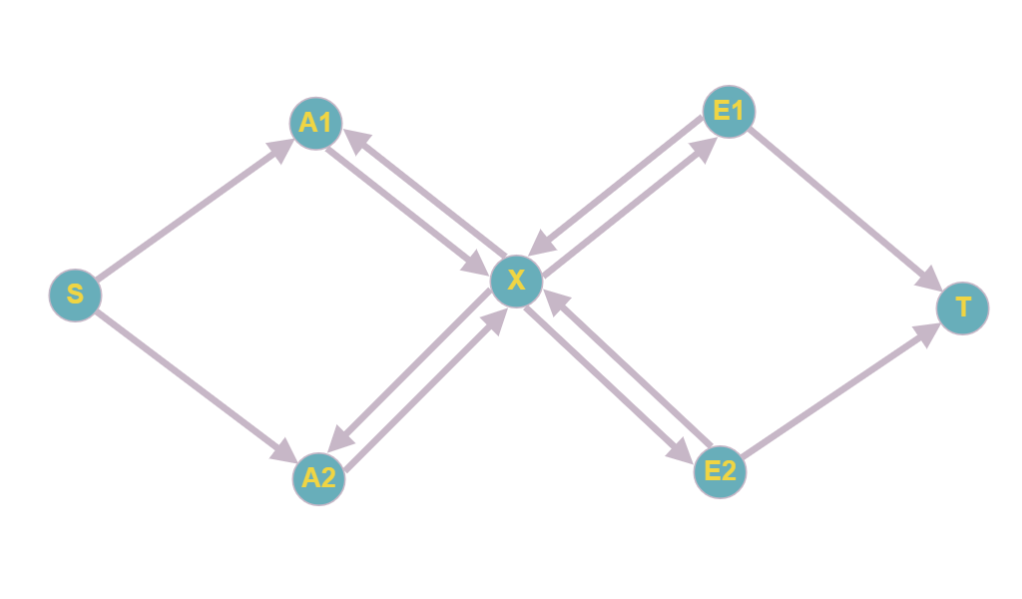
\includegraphics[width=15cm]{Imagenes/Ej1c.png}
\caption{Grafo 2}
\end{figure}

En el Grafo 2, se puede observar que el flujo máximo es 2, pero con poner un único divulgador en el vértice del medio el problema se solucionaría. Esto se debe a que los divulgadores se ubican en los vértices y no en los ejes. Es decir, los vértices deberían tener capacidades también. Entonces se decidió poner capacidad 1 a los vértices. Así se armó un grafo nuevo, partiendo cada nodo $v$ en $v_{in}$ y $v_{out}$ (conectados entre si por un eje dirigido de $in$ a $out$). Se conectó la fuente a los $in$ de los alumnos, se conectó el sumidero a los $out$ de las escuelas. La idea es que al $in$ lleguen todos los ejes entrantes y que del $out$ salgan todos los salientes. Quedaría entonces el Grafo 3.

\begin{figure}[H]
\centering
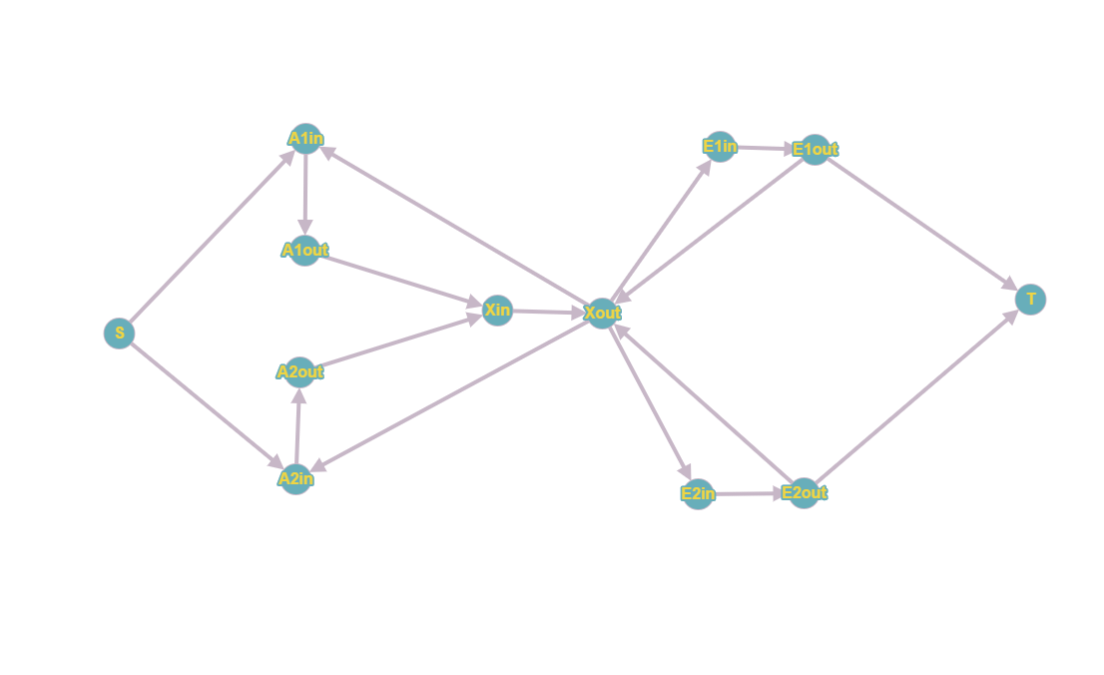
\includegraphics[width=15cm]{Imagenes/Ej1b.png}
\caption{Grafo 3}
\end{figure}

En el Grafo 3, se puede ver que el flujo máximo va a dar 1. Esto se debe a que el eje de $X_{in}$ a $X_{out}$ es el cuello de botella. El corte mínimo sería el que se puede ver en la siguiente imagen.

\begin{figure}[H]
\centering
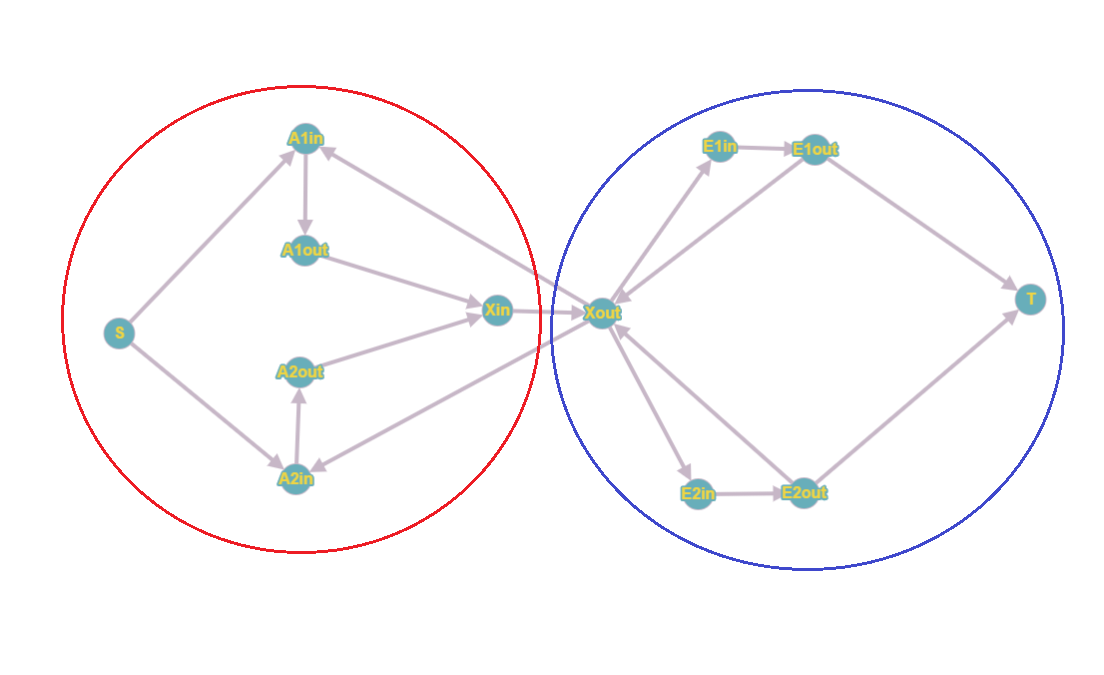
\includegraphics[width=15cm]{Imagenes/Ej1d.png}
\caption{Corte Mínimo del Grafo 3}
\end{figure}

Al armar el grafo de esta forma, ahora se tienen en cuenta los vértices, por lo que el corte mínimo va a solucionar efectivamente el problema. Este sería, el corte que separa la fuente y el sumidero y minimiza el peso total de los ejes que salen del lado de la fuente hacia el lado del sumidero.

Más formalmente, dado el grafo original $G$ $=$ $(V,E)$, se arma uno nuevo, $G' = (V_{in} \cup V_{out} \cup \{s,t\}, E')$. Para modelar las capacidades de los nodos, se dividió $V$ en dos conjuntos disjuntos $V_{in}$ y $V_{out}$. Cada vértice de $v_i \in V$ se corresponde con un un $v_{iin} \in V_{in}$ y un $v_{iout} \in V_{out}$. 

\begin{itemize}
\item Por cada vértice $v \in V$ se agrega a $E'$ el eje $(v_{in},v_{out})$.
\item Por cada uno de los ejes $(u,v) \in E$, se agregan los ejes $(u_{out}, v_{in})$ y $(v_{out}, u_{in})$.
\item Por cada vértice $a \in A$ se agrega a $E'$ un eje $(s,a_{in})$.
\item Por cada vértice $e \in Esc$ se agrega a $E'$ un eje $(e_{out},t)$.
\end{itemize}

%Quizás mencionar algo más sobre por qué se soluciona el problema.


\subsubsection{Implementación}

Se adjunta un pseudocódigo del algoritmo implementado.

\begin{verbatim}
    ejercicio2(grafo G){
        G' <- armarGrafo(G)
        res <- edmondsKarp(G')
        return res
    }
\end{verbatim}

Donde la función \texttt{armarGrafo} arma el grafo del modelado. Esto es, conectando los alumnos a la fuente y las escuelas al sumidero. Luego por cada eje, cambia el eje $(u,v)$ por $(u_{out}, v_{in})$ y $(v_{out}, u_{in})$.

Se implementó luego el algoritmo de Edmonds-Karp para resolver el problema de flujo máximo (que resuelve el problema de corte mínimo).

%Hablar más de Edmonds-Karp (EZE.SUMMON())


\subsubsection{Complejidad}

En esta sección se comentará la complejidad del algoritmo implementado. Primero se analizará la complejidad del armado del grafo. El grafo se va armando a medida se va leyendo la entrada, implementado con listas de adyacencia. Esto es:

\begin{itemize}
\item Primero se lee $N$ y se arma un vector de tamaño $2*N + 2$ (un $in$ y un $out$ por cada vértice original más fuente y sumidero). Esto es del orden de $O(N)$.
\item Por cada vértice que se lee de la entrada, se conecta su $in$ con su $out$. Si se trata de una escuela, se conecta su $out$ al sumidero y si se trata de un alumno, se conecta la fuente a su $in$. Esto es del orden de $O(1)$ y como se hace una vez por vértice, este paso es del orden de $O(N)$.
\item Por cada eje $(u,v)$ que se lee de la entrada, se conecta $(u_{out}$ con $v_{in})$ y $(v_{out}$ con $u_{in})$. Esto es $O(1)$ y como se hace una vez por cada eje, este paso es del orden de $O(M)$.
\end{itemize}

Esto deja una complejidad total de $O(N+M)$ para el armado del grafo. Luego le sigue el algoritmo de Edmonds-Karp. Este tiene una complejidad de $O(M^2N)$. Cabe mencionar que el grafo que se arma tiene $2*N+2$ vértices y $2*M + A + E + N$ ejes (con $A$ cantidad de alumnos y $E$ cantidad de escuelas). 

%% EZE.SUMMON() habla de la complejidad de Edmonds-Karp si queres.

Como el grafo original es conexo, tiene al menos $N-1$ ejes, esto es,  $O(N) \subseteq O(M)$. Además, $O(A) \subseteq O(N)$ y $O(E) \subseteq O(N)$ porque $A+E \leq N$. Entonces $O(2*M + A + E + N) \subseteq$ $O(M)$. Además, el grafo nuevo tiene $2*N+2$ vértices, es decir, $O(N)$ vértices. 

Por lo tanto, el nuevo grafo tiene $O(N)$ vértices y $O(M)$ ejes, por lo que la complejidad de Edmonds-Karp es de $O(M^2N)$.

Entonces la complejidad total del algoritmo es $O(M^2N + N + M)$. Como $N > 0$ y $M>0$, $O(N+M) \subseteq O(M^2N)$. Por lo tanto, la complejidad total del algoritmo es de $O(M^2N)$.